\documentclass{article}
\usepackage{graphicx}
\usepackage[margin=1.5cm]{geometry}
\usepackage{amsmath}
\usepackage{fancyvrb}
\usepackage{url}

\begin{document}

\title{Synopsis - Week 11 and 12 Integrated Project: ADC, DAC, and The Nyquist Frequency}
\author{Prof. Jordan C. Hanson}

\maketitle

\section{ADC and DAC Setup}

Peripheral modules from Digilent are called Pmods.  Pmods allow peripheral devices to connect and interact with the PYNQ-Z1 system and give it special abilities.  In this lab, we will encounter analog-to-digital converters (ADCs) and digital-to-analog converters (DACs).  In lecture, we will cover the Flash ADC.  An ADC samples and digitizes analog voltages, and provides digital binary output representing the analog signal.  A DAC converts digital binary numbers to an analog voltage on the output.  \textit{In this lab activity, we will produce analog voltages via a DAC and feed them into an ADC.}  Figure \ref{fig:setup1} at the back of this document depicts the setup.

\section{Create Code to Send and Plot a Sine Wave}

\subsection{Set up the system correctly}

Set up a new Jupyter workbook with the following libraries and toos:

\begin{verbatim}
#Setup programmable logic, including Pmods for DAC and ADC, and other libraries
%matplotlib inline
import matplotlib.pyplot as plot
from time import sleep
import numpy as np
import matplotlib.pyplot as plt
from pynq.lib import Pmod_ADC, Pmod_DAC
from pynq.overlays.base import BaseOverlay
ol = BaseOverlay("base.bit")
dac = Pmod_DAC(ol.PMODB)
adc = Pmod_ADC(ol.PMODA)
\end{verbatim}

The above code imports matplotlib, to graph the ADC output from the DAC input.  We also program the firmware to handle PMODA controlling the ADC, while PMODB controls the DAC.  They are connected physically by a wire.  Numpy is imported for math utilities, including creating vectors of data.

\subsection{Send a Sine Wave through the DAC to the ADC}

The following code defines a frequency $f$, an amplitude $A$, a DC offset $B$, a list of times $t$, and computes the sine wave according to

\begin{equation}
v(t) = A\sin(2\pi ft) + B
\end{equation}

The interesting part is that we must define \textit{a list} of times, spaced by $\Delta t$.  The \textit{sampling frequency} is $f_s = 1/\Delta t$.  Each sine wave value is sent over the line from the DAC to the ADC, value by value, and system sleeps for $\Delta t$ seconds.  The \verb+samples+ variable captures the ADC output.

\begin{verbatim}
#Transmission loop
sampling_frequency = 10.0 #Units: Hertz
delta_t = 1.0/sampling_frequency #Units: seconds
t_max = 10.0 #Units: seconds
times = np.arange(0, t_max, delta_t)
dc_offset = 1.0 #Units: volts
amplitude = 0.5 #Units: volts
frequency = 0.5 #Units: Hertz
samples = []
for t in times:
    dac.write(amplitude*np.sin(2.0*3.14159*frequency*t)+dc_offset)
    sleep(delta_t)
    samples.append(adc.read())
\end{verbatim}

\subsection{Plotting the Results}

In the following code, a plot is created from the pyplot module from the matplotlib library.  The list of times defined in the last section is plotted on the x-axis, and the ADC voltages are plotted on the y-axis.  The title of the plot should display the sampling frequency and sine wave frequency.

\begin{verbatim}
#Plotting section
plot.plot(times,samples,'-o')
plotTitle = "Frequency: "+str(frequency)+" Hz, Sampling Frequency: "+str(sampling_frequency)+" Hz"
plot.title(plotTitle)
plot.xlabel('Time (seconds)')
plot.ylabel('Amplitude (Volts)')
plot.grid(True, which='both') 
plot.legend(loc='upper left')
plot.axis([0, t_max, 0, 2.0])
plot.show()
\end{verbatim}

\subsection{Questions to be Answered}

\begin{enumerate}
\item What happens when the frequency of the sine wave is greater than half of the sampling frequency?  Create a plot that (a) sets the sine wave frequency equal to one-half of the sampling frequency.  (b) Create plots that push the sine wave frequency to values greater than one-half of the sampling frequency.  What do you observe? \\ \vspace{3cm}
\item While respecting the Nyquist-Shannon limit ($f \leq f_s/2$), push the frequency of the sine wave into the MHz regime.  How high can you make the sine wave frequency before you start to notice changes in the sine wave amplitude?  What happens to the sine wave amplitude?
\end{enumerate}

\begin{figure}
\centering
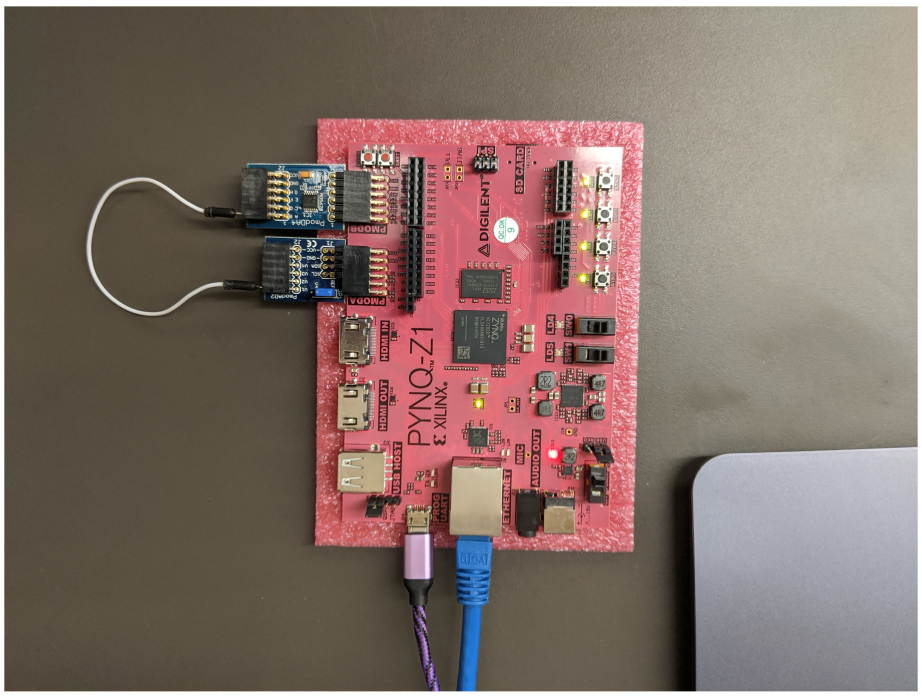
\includegraphics[width=0.85\textwidth]{pmod.png}
\caption{\label{fig:setup1} The PYNQ-Z1 board, along with the AD2 and DA4 Pmods.  The blue objects are the Pmods: the lower one is the ADC and the upper is the DAC.  The ADC has 12-bits of resolution and a range of 0-2V.}
\end{figure}

\end{document}
